\section{Performance Evaluation}
\paragraph{Needs-Analysis Results: Separate from System Performance.}
The three survey exports contain 66, 13 and 7 submissions, respectively (86 total). One explicit non-consenting submission is excluded. Of the 85 affirmative-consent submissions, four report an age below 18 and two omit age. The primary analysis therefore includes 79 adult submissions. No identical complete submission was found after aligning the service blocks, but this does not establish unique participant identities. The analysis is reproducible from the private archive using \path{scripts/analyze_needs_survey.py}; public artifacts contain aggregate counts, inclusion rules and an archive hash only.

The sample is concentrated among younger adults and men: 63/79 (79.7\%) report age 18--25, and 73/79 (92.4\%) report male gender. Recruitment and invitation counts are unavailable. Findings describe this responding sample and must not be extrapolated to all Bangladeshi citizens. They are not results from the 30-question chatbot experiment.

\begin{table}[htbp]\centering\small
\caption{Needs-analysis responses among consenting adults. Denominators exclude blank answers to each item.}\label{tab:needs-survey}
\begin{tabularx}{\linewidth}{Xr}\toprule
Response & Count / valid responses (percentage)\\\midrule
Would use the proposed AI assistant & 55/77 (71.4\%)\\
Would not use it & 13/77 (16.9\%)\\
Unsure about using it & 9/77 (11.7\%)\\
Would recheck even verified information & 42/76 (55.3\%)\\
Bangla would be more comfortable & 19/77 (24.7\%)\\
Either Bangla or English acceptable & 50/77 (64.9\%)\\
Would recommend if it works well & 67/76 (88.2\%)\\
\bottomrule\end{tabularx}\end{table}

Among valid willingness responses, 55/77 (71.4\%) would use the prospective assistant, 13/77 (16.9\%) would not and 9/77 (11.7\%) were unsure. The two missing responses are not counted as either acceptance or rejection. For trust in verified information, 30/76 (39.5\%) answered yes, 4/76 (5.3\%) no and 42/76 (55.3\%) would recheck. Positive willingness and cautious trust can coexist: the questionnaire supports the need for helpful information with verification opportunities, not unrestricted reliance on AI.

Figures~\ref{fig:survey-trust} and \ref{fig:survey-features} visualize these preferences and the requested kinds of assistance.

\begin{figure}[htbp]\centering
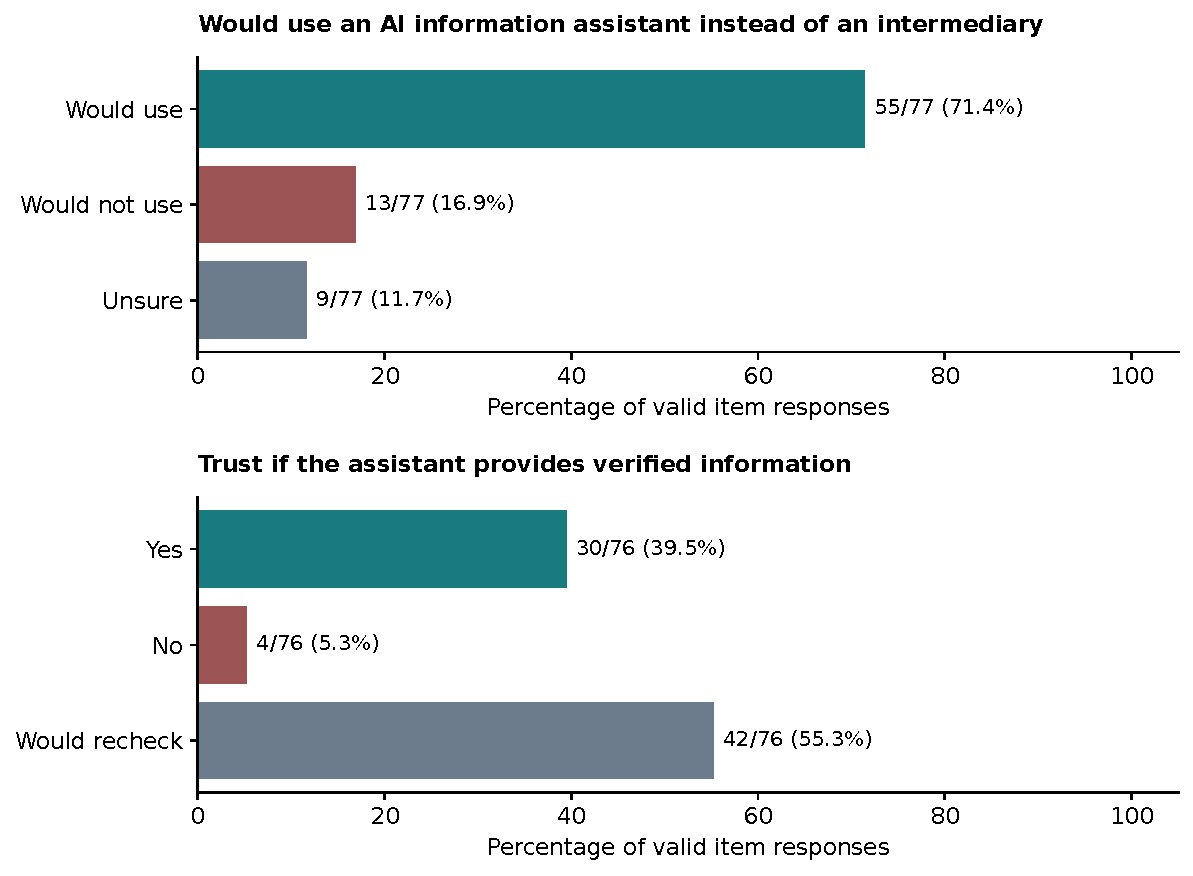
\includegraphics[width=\linewidth]{generated/survey_willingness_trust.pdf}
\caption{Stated willingness and conditional trust in the needs-analysis questionnaire. Only consenting adult submissions are included; denominators differ because of missing answers.}\label{fig:survey-trust}
\end{figure}

\begin{figure}[htbp]\centering
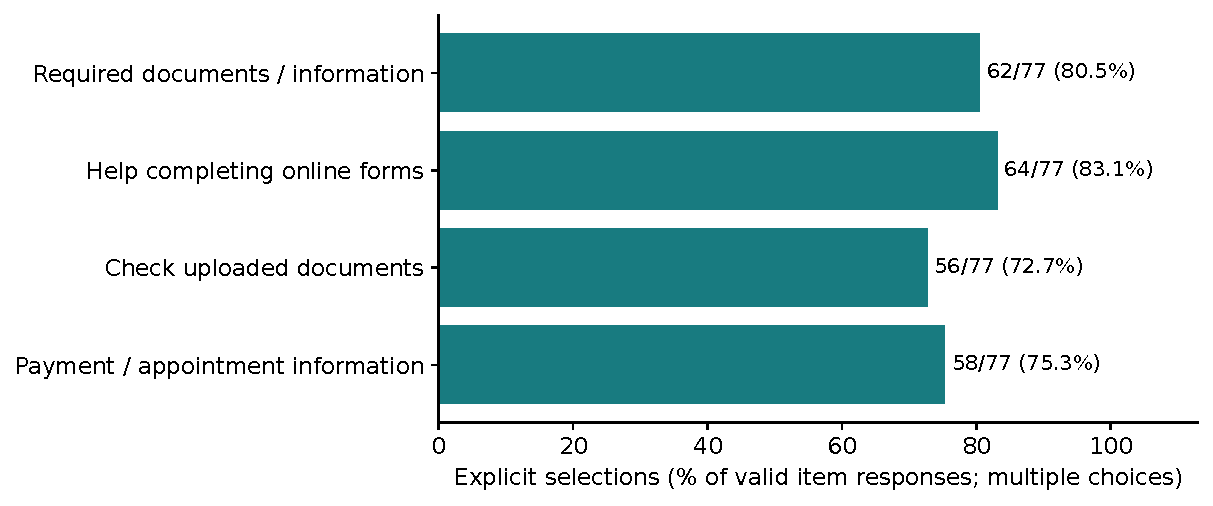
\includegraphics[width=\linewidth]{generated/survey_features.pdf}
\caption{Requested assistance, based on explicit selections among 77 valid responses. Multiple choices were allowed. One ``all options'' response is not expanded, so explicit-choice counts are conservative. Requested features are not necessarily implemented capabilities.}\label{fig:survey-features}
\end{figure}

Required-document information (80.5\%) and payment/appointment information (75.3\%) align with the implemented question-answering scope. Form-completion assistance (83.1\%) and uploaded-document checking (72.7\%) indicate additional expectations beyond that scope. This distinction prevents reporting questionnaire demand as proof that the system already satisfies every requested function.

The language item does not establish a majority preference for Bangla-only operation. Nineteen of 77 respondents (24.7\%) said Bangla would be more comfortable, 50 (64.9\%) accepted either Bangla or English and eight (10.4\%) answered no. Bangla-focused evaluation is therefore a project scope decision consistent with part of the expressed need, rather than a requirement endorsed exclusively by most respondents. Conditional recommendation was positive for 67/76 (88.2\%), but the question assumes the assistant works well; it is not satisfaction measured after using CivicRAG.

\paragraph{Experimental Design.}
The primary comparison uses the same 30 Bangla questions and domain-scoped corpus for Simple RAG and CivicRAG. Each system produced one saved answer per question using Qwen3:8b, the matched generation prompt and the same context and output limits. Simple RAG uses dense retrieval without fusion, reranking or applicability selection; CivicRAG includes these stages as described in Section 4.2. The comparison measures the combined configuration difference, not the isolated contribution of each component.

There are ten questions each for birth registration, passport and driving-licence services. All are labelled direct in the saved plan. They concern requirements, fees, time, application, correction, renewal, replacement and status. They were reused during development, so these are development-set results rather than estimates on an unseen benchmark. The source answers and hashes are preserved in the evaluation archive. No answers were regenerated for scoring or thesis preparation.

\paragraph{Operational Outcomes.}
Table~\ref{tab:operational-final} reports saved latency and context size. Both systems completed 30 requests; completion is not a correctness label.
\begin{table}[htbp]\centering\small
\caption{Operational measurements for the matched 30-question runs. Times are seconds; runs occurred separately.}\label{tab:operational-final}
\begin{tabularx}{\linewidth}{Xrr}\toprule
Measure & Simple RAG & CivicRAG\\\midrule
Completed requests & 30 & 30\\
Mean elapsed time & 193.699 & 181.823\\
Median elapsed time & 181.060 & 161.845\\
95th percentile & 319.910 & 285.100\\
Mean supplied passages & 6.000 & 4.900\\
Mean context characters & 5218.900 & 3948.033\\
Mean Bangla-letter fraction & 0.935 & 0.933\\\bottomrule
\end{tabularx}\end{table}
CivicRAG supplied fewer passages and characters on average. Its saved mean latency was also lower, but machine load, thermal conditions and initialization were not controlled across the two runs. Therefore the table does not establish a hardware-normalized speed advantage. Bangla-letter fraction measures script use after removing the source footer; it is not a fluency or correctness score.

\paragraph{Completed RAGAS and Custom Context Evaluation.}
The evaluator uses RAGAS 0.2.15 and actual supplied answer contexts, not every retrieved candidate \cite{ragas}. The official versioned metrics reference documents the metric interfaces \cite{ragas_docs}; its cited documentation snapshot is 0.2.12, whereas the recorded installed package is 0.2.15. There are $30\times2\times3=180$ completed metric scores, all valid, with no missing final scores. The appended Sources footer is removed before evaluation; response wording is otherwise preserved.

Faithfulness estimates support for the response statements in the supplied context:
\begin{equation}
F=\frac{\sum_{j=1}^{m}\mathbf{1}[a_j\text{ is supported by context}]}{m}.
\end{equation}
Here $a_j$ is a judge-extracted statement. This tests textual support, not current legal validity. Answer relevancy reconstructs three questions from a response and compares their BGE-M3 embeddings with the original question, with the metric's noncommittal-response handling. It is not similarity to a reviewed reference answer.

The third measure is a custom binary RAGAS AspectCritic. It asks whether most supplied context concerns the requested service, procedure and conditions, instructing the judge to ignore the response. Each context set receives 0 or 1. Its mean is therefore a share of positively judged context sets, not passage-level context precision or recall.

The judge is Qwen3:8b, also the answer generator. The evaluation uses temperature zero, seed 20260924, non-thinking mode, a 16,384-token context window and a 4,096-token output allowance. Stock evaluation prompts are applied to Bangla content. This completed computation remains an exploratory self-judge evaluation: a fixed seed and valid output format do not make the judge independent or its scores equivalent to factual accuracy.

Table~\ref{tab:ragas-final} presents the completed means, and Figure~\ref{fig:ragas-final} visualizes the same values.
\begin{table}[htbp]\centering\small
\caption{Completed saved-answer evaluation: Qwen3 self-judge scores, not independent accuracy.}\label{tab:ragas-final}
\begin{tabularx}{\linewidth}{Xrrrr}\toprule
Metric & Simple & CivicRAG & $\Delta$ & Pairs\\\midrule
Faithfulness & 0.7983 & 0.7323 & -0.0660 & 30\\
Answer relevancy & 0.8460 & 0.8375 & -0.0085 & 30\\
Custom context relevance & 0.9333 & 0.9667 & +0.0333 & 30\\
\bottomrule\end{tabularx}\end{table}

\begin{figure}[htbp]\centering
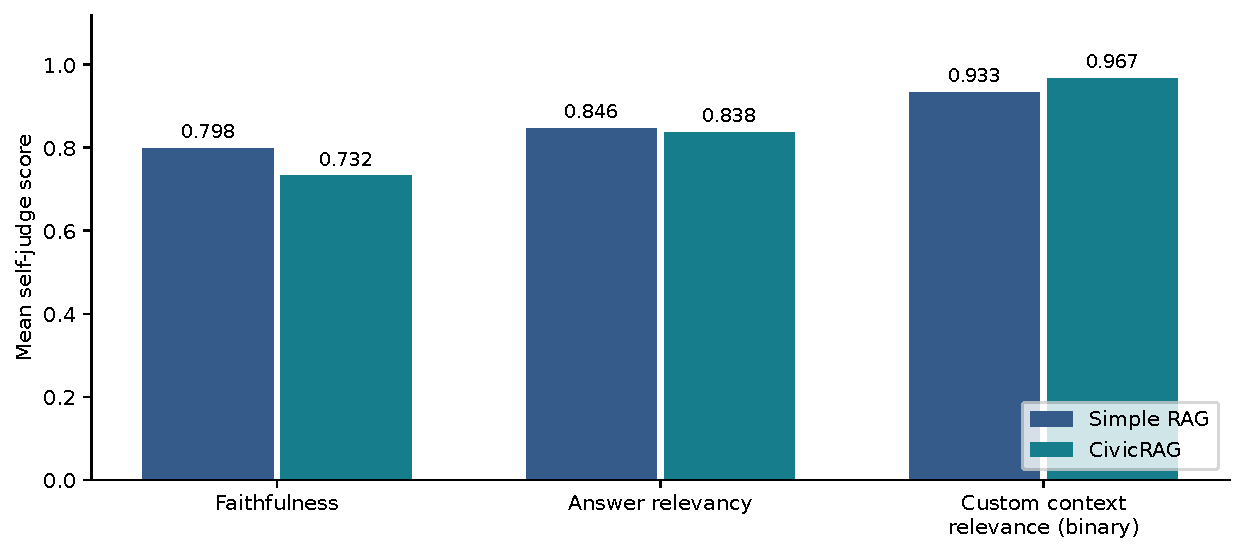
\includegraphics[width=\linewidth]{generated/ragas_final_chart.pdf}
\caption{Completed local self-judge scores for matched saved answers, with 30 valid scores per system and measure. Custom context relevance is binary and distinct from standard context precision/recall.}\label{fig:ragas-final}
\end{figure}
Simple RAG has higher mean faithfulness (0.7983 versus 0.7323) and slightly higher answer relevancy (0.8460 versus 0.8375). CivicRAG has higher custom context relevance (0.9667 versus 0.9333), corresponding to 29 versus 28 positive context-set judgments. These results describe different aspects of behaviour and do not establish a single overall winner.

\paragraph{Provisional Retrieval-Only Evaluation.}
A separate experiment compares BM25-only, dense-only and weighted Hybrid RRF on the same 30 questions before reranking, registration boosts and evidence selection. No answer generation occurs in this experiment. The top-five result union for each question forms a relevance pool; an assistant reviewed 309 question/passage pairs representing 192 unique passages. The labels are 105 relevant, 199 irrelevant and five uncertain.

These are unblinded, single-assistant labels, not independently human-verified ground truth or original-document legal verification. Four questions containing uncertain labels are excluded from all three methods, leaving 26 for Hit, Precision and MRR. One further question has no relevant passage in its judged pool; pooled Recall and nDCG therefore use 25 questions. This exclusion does not prove that the entire database lacks useful evidence.

The following equations specify the ranked-retrieval measures used in this study. Let $z_{qi}$ indicate whether the chunk at rank $i$ is labelled relevant, and let $R_q$ be the relevant IDs in the judged pool. For each eligible question:
\begin{align}
\mathrm{Precision@5}(q)&=\frac{1}{5}\sum_{i=1}^{5}z_{qi},\\
\mathrm{Hit@k}(q)&=\mathbf{1}\left[\sum_{i=1}^{k}z_{qi}>0\right],\quad k\in\{1,5\},\\
\mathrm{RR@5}(q)&=\begin{cases}1/r_q,&r_q\leq5,\\0,&\text{no relevant result in top five},\end{cases}\\
\mathrm{Recall@5}_{\mathrm{pool}}(q)&=\frac{|\mathrm{Top5}(q)\cap R_q|}{|R_q|}.
\end{align}
MRR@5 averages RR@5 over eligible questions. Recall is undefined for an empty relevant pool. Following the normalized cumulative-gain framework \cite{ndcg}, with binary relevance the discounted measure is
\begin{equation}
\mathrm{nDCG@5}_{\mathrm{pool}}(q)=
\frac{\sum_{i=1}^{5}z_{qi}/\log_2(i+1)}
{\sum_{i=1}^{\min(5,|R_q|)}1/\log_2(i+1)}.
\end{equation}
Incomplete relevance judgments can affect retrieval evaluation \cite{incompletejudgments}. Pooled Recall and nDCG use only relevant passages found in the pooled rankings, not exhaustive corpus labels. Missing retrieved positions contribute zero to Precision's fixed denominator of five. Near-duplicate IDs remain distinct scoring units.

Table~\ref{tab:retrieval-overall} gives overall results. Asterisks denote pooled, rather than corpus-wide, relevance denominators.
\begin{table}[htbp]\centering\small
\caption{Overall: provisional retrieval-only scores with assistant-reviewed labels. Hit, precision and MRR use 26 questions; pooled recall and nDCG use 25.}\label{tab:retrieval-overall}
\begin{tabularx}{\linewidth}{Xrrrrrr}\toprule
Method & H@1 & H@5 & P@5 & R@5* & MRR@5 & nDCG@5*\\\midrule
BM25 & 0.3077 & 0.6538 & 0.2769 & 0.3523 & 0.4179 & 0.3553\\
Dense & 0.6923 & 0.8846 & 0.5000 & 0.7221 & 0.7821 & 0.7156\\
Hybrid RRF & 0.4231 & 0.8846 & 0.4462 & 0.6173 & 0.6263 & 0.5863\\
\bottomrule\end{tabularx}\end{table}

Dense retrieval leads on Hit@1, Precision@5, pooled Recall@5, MRR@5 and pooled nDCG@5. Dense and Hybrid RRF tie on overall Hit@5 (0.8846). Thus adding BM25 through these fixed fusion weights does not improve every first-stage ranking measure. These provisional results neither invalidate all uses of hybrid retrieval nor prove the complete answer pipeline inferior: later reranking and selection are deliberately absent.

\section{Analysis of Design Solutions}
\paragraph{What the Diagnostics Show.}
Generation-only trials supplied manually inspected passages for three known questions, then varied evidence order and added distracting passages. Better responses with relevant-only evidence still used the LLM; they were not controlled template answers. The trials showed why context selection deserved attention, but did not establish an automatic selector's performance on arbitrary queries. This distinction is consistent with research separating retrieval quality from context use \cite{trase,lostmiddle}.

The final matched comparison tests the automatically selected evidence rather than those manually curated diagnostic contexts. The RAGAS result is mixed: more positively judged context sets coexist with lower mean faithfulness. One possible explanation is that the remaining context contains conditions the generator combines incorrectly, but the current comparison does not isolate that mechanism. A context score cannot replace inspection of the answer.

\paragraph{Illustrative Outputs Provided by the Authors.}
The following three examples were supplied with the thesis revision request. All are reported with route \code{llm_selected_evidence}. Their reported times differ from the frozen comparison rows, whose corresponding elapsed times are 204.17, 147.21 and 180.81 seconds. We therefore retain the examples as author-supplied qualitative demonstrations and do not insert their timings or wording into the aggregate benchmark. The excerpts below preserve selected supplied sentences; they are neither gold answers nor current official instructions.

For passport services, the question is \bn{পাসপোর্ট হারিয়ে গেলে কী করতে হবে?}, with a supplied time of 240.45 seconds. The response includes:
\begin{quote}
\bn{হারানো পাসপোর্টের ক্ষেত্রে অথবা চুরি হলে দ্রুত নিকটস্থ থানায় জিডি (GD) করতে হবে।}\\
\bn{পুনরায় পাসপোর্টের জন্য আবেদনের সময় পূর্ববর্তী পাসপোর্টের ফটোকপি এবং জিডি কপি সহ আবেদনপত্র দাখিল করতে হবে।}
\end{quote}
The response addresses replacement rather than unrelated passport collection. Its additional identity-document and occupation-specific requirements still need condition-by-condition verification: a useful core instruction does not make every appended requirement applicable to every applicant. The route confirms model generation after selection, not independent validation.

For birth registration, the question is \bn{জন্মনিবন্ধন অনলাইনে কীভাবে করব?}, with a supplied time of 176.82 seconds. The response directs the user to \url{https://bdris.gov.bd} and includes:
\begin{quote}
\bn{সমস্ত প্রয়োজনীয় তথ্য পূরণ করুন এবং আবেদন সাবমিট করুন।}\\
\bn{দুইটি জমজ সন্তানের ক্ষেত্রে, প্রথম সন্তানের জন্ম নিবন্ধন শেষ হওয়ার পরে দ্বিতীয় সন্তানের জন্ম নিবন্ধন করতে হবে।}
\end{quote}
The portal-oriented answer aligns with an online application question. However, the unsolicited twin-specific condition shows that source-related content can enter a general answer without being requested. This example illustrates the need to separate general steps from exceptional cases, rather than assuming additional detail is always an improvement.

For BRTA, the question is \bn{BRTA-এর ড্রাইভিং পরীক্ষায় কী কী থাকে?}, with a supplied time of 183.21 seconds. The response lists:
\begin{quote}
\bn{লিখিত পরীক্ষা}\\
\bn{মৌখিক পরীক্ষা}\\
\bn{ব্যবহারিক পরীক্ষা}
\end{quote}
The short list is more directly usable than a long legal extract. Nevertheless, the actual comparison trace discussed in Section 4.4 contains neighbouring licence topics, so this apparently clear answer is not evidence that all selected passages were applicable. Its supplied demonstration wording also differs slightly from the stored response. Across the three examples, local response latency remains substantial for interactive use.

\paragraph{Paired Answer Observations.}
Saved answers show both useful changes and regressions. Passport-document and fee answers become more task-aligned in CivicRAG, whereas the birth-registration timing response substitutes an application deadline for a processing time. Driving-licence status remains problematic. These examples explain why the evaluation retains multiple measures rather than declaring correctness from answer length or source IDs.

The authors' domain-informed preference for some more complete answers is useful qualitative feedback. Without a completed consistent review sheet, it is not converted into an aggregate expert accuracy percentage. Likewise, automatically assigned context labels cannot be relabelled as human judgments.

\section{Final Design Adjustments}
The evaluated configuration includes automatic applicability screening and the compatible-family ordering correction. Previously, compatible sibling fee sections could be appended after other candidates and then excluded by the context budget. Grouping them near the first eligible anchor changed the selected IDs for one question in a saved 30-case replay. This is a measured replay observation, not proof of general answer improvement.

The main CivicRAG answer file was generated after that correction. Its corpus, prompts and configuration were frozen for the matched comparison. No architecture change, model retraining or new answer generation was introduced while computing the reported metrics. The selected-evidence path bypasses older controlled-answer templates; the qualitative examples should not be described as those templates' output.

Documentation refinements, including birth-registration terminology and the architecture diagrams, do not alter the underlying collection identifiers, code or saved results. The label retained in stored files is a provenance identifier, not an expansion of the evaluated service scope.

\section{Statistical Analysis}
Survey percentages use valid item responses rather than a fixed denominator for every question. Unknown recruitment, demographic concentration and unverified repeat participation prevent nationally representative inference. These descriptive needs-analysis statistics are separate from the paired system results.

Statistical conclusions depend on the evaluation design and the assumptions of the selected procedure \cite{drorstats}. Our paired resampling describes uncertainty within the saved question set; it does not establish external validity. For each automatic metric, define $\delta_q=s_{\mathrm{Civic},q}-s_{\mathrm{Simple},q}$. All 30 pairs have valid scores. The saved evaluator resamples the 30 paired differences with replacement 2,000 times, using seed 20260924, and reports empirical 95\% intervals. Table~\ref{tab:ragas-intervals} reproduces those saved intervals rather than recomputing a different protocol.
\begin{table}[htbp]\centering\small
\caption{Paired CivicRAG minus Simple RAG differences with descriptive bootstrap intervals.}\label{tab:ragas-intervals}
\begin{tabularx}{\linewidth}{Xrr}\toprule
Metric & Mean $\Delta$ & 95\% interval\\\midrule
Faithfulness & -0.0660 & [-0.1787, 0.0410]\\
Answer relevancy & -0.0085 & [-0.0347, 0.0194]\\
Custom context relevance & +0.0333 & [0.0000, 0.1000]\\
\bottomrule\end{tabularx}\end{table}

The faithfulness and answer-relevancy intervals span zero; the custom binary context-relevance interval reaches zero. They reflect question resampling within this reused set, not judge calibration, repeated-generation variance or corpus representativeness. We therefore make no statistically established claim of overall factual superiority.

Per-domain retrieval results are shown in Tables~\ref{tab:retrieval-passport}--\ref{tab:retrieval-brta}. Values are question-level means over eligible questions; the overall score weights the eligible questions, not the three domain means equally.
\begin{table}[htbp]\centering\small
\caption{Passport: provisional retrieval-only scores with assistant-reviewed labels. Hit, precision and MRR use 8 questions; pooled recall and nDCG use 8.}\label{tab:retrieval-passport}
\begin{tabularx}{\linewidth}{Xrrrrrr}\toprule
Method & H@1 & H@5 & P@5 & R@5* & MRR@5 & nDCG@5*\\\midrule
BM25 & 0.5000 & 0.7500 & 0.3000 & 0.3088 & 0.5833 & 0.3798\\
Dense & 0.7500 & 1.0000 & 0.6500 & 0.7173 & 0.8750 & 0.7607\\
Hybrid RRF & 0.3750 & 1.0000 & 0.4750 & 0.5253 & 0.6562 & 0.5328\\
\bottomrule\end{tabularx}\end{table}

\begin{table}[htbp]\centering\small
\caption{Birth registration: provisional retrieval-only scores with assistant-reviewed labels. Hit, precision and MRR use 9 questions; pooled recall and nDCG use 9.}\label{tab:retrieval-birth_death_registration}
\begin{tabularx}{\linewidth}{Xrrrrrr}\toprule
Method & H@1 & H@5 & P@5 & R@5* & MRR@5 & nDCG@5*\\\midrule
BM25 & 0.3333 & 0.6667 & 0.2667 & 0.4370 & 0.4296 & 0.3938\\
Dense & 0.5556 & 0.7778 & 0.4222 & 0.6963 & 0.6481 & 0.6173\\
Hybrid RRF & 0.4444 & 0.8889 & 0.4222 & 0.6685 & 0.6148 & 0.5882\\
\bottomrule\end{tabularx}\end{table}

\begin{table}[htbp]\centering\small
\caption{BRTA: provisional retrieval-only scores with assistant-reviewed labels. Hit, precision and MRR use 9 questions; pooled recall and nDCG use 8.}\label{tab:retrieval-brta}
\begin{tabularx}{\linewidth}{Xrrrrrr}\toprule
Method & H@1 & H@5 & P@5 & R@5* & MRR@5 & nDCG@5*\\\midrule
BM25 & 0.1111 & 0.5556 & 0.2667 & 0.3006 & 0.2593 & 0.2875\\
Dense & 0.7778 & 0.8889 & 0.4444 & 0.7560 & 0.8333 & 0.7809\\
Hybrid RRF & 0.4444 & 0.7778 & 0.4444 & 0.6518 & 0.6111 & 0.6377\\
\bottomrule\end{tabularx}\end{table}

Dense and hybrid search both achieve passport Hit@5 of 1.0000 on eight eligible questions. For birth registration, hybrid Hit@5 is 0.8889 versus dense 0.7778 on nine questions, while dense retains stronger MRR. In BRTA, dense Hit@5 is 0.8889 versus hybrid 0.7778. These differences show why per-domain analysis is useful, but the small eligible samples and provisional labels limit generalization.

Uncertain questions excluded consistently across methods concern passport fees, passport renewal, birth-date proof and licence renewal. The licence-status pool contains no labelled relevant passage and is omitted only from pooled Recall/nDCG denominators. Uncertain labels are not treated as irrelevant, and missing scores are not replaced with zeros.

\paragraph{Exploratory Overnight Labeling.}
A separate Qwen3 labeling job completed 455 judgments over saved candidate and supplied passages: 176 relevant, 191 irrelevant and 88 uncertain. It hides system names, ranks and responses from the judge, but shares the generator's model family. Under its stricter requirement for complete, nonempty relevant pools, only one of 30 questions is scorable. This is a completed labeling run with incomplete adjudication, not a completed 30-question retrieval benchmark.

The single scorable passport question has Precision@5 of 0.8 for Simple RAG and 1.0 for CivicRAG, with pooled Recall@5 of 0.8 and 1.0. Those numbers cannot support a system-level conclusion. This pool differs from the three-retriever top-five pool and its labels were not merged with the assistant-reviewed study. In particular, 455 judgments and 309 judgments are not two versions of one gold dataset.

\section{Comparisons and Relationships}
The secondary model runs use the same selected-evidence configuration and matching ordered context content. Table~\ref{tab:models-final} summarizes operational outcomes; no equivalent RAGAS comparison is claimed for these secondary models.
\begin{table}[htbp]\centering\small
\caption{Secondary generator runs on the selected-evidence configuration. Language rejections are operational events, not factual error counts.}\label{tab:models-final}
\begin{tabularx}{\linewidth}{Xrrr}\toprule
Model & Requests & Mean seconds & Language rejections\\\midrule
Qwen3:8b & 30 & 181.82 & 0\\
Llama3 & 30 & 148.64 & 7\\
Qwen2.5:7b & 30 & 147.38 & 1\\\bottomrule
\end{tabularx}\end{table}
Qwen3 was a practical choice for the main comparison, not an established best model for Bangla. Its model family supports the local deployment \cite{qwen3}; the observed outcomes belong to these particular recorded runs. Language rejection does not prove a response was factually wrong, and acceptance does not prove it was correct.

The comparison has two distinct levels. The answer-pipeline experiment holds generator settings fixed and varies retrieval plus later evidence processing. The retrieval-only experiment compares ranking before those later stages. A strong first-stage dense ranking can coexist with a helpful hybrid-pipeline answer on an individual question; conversely, a positive context-set judgment can coexist with an unsupported generated statement.

The earlier 58-question registration-focused retrieval study uses different questions and labels and is not pooled into the current tables. NextRAG informs the method \cite{nextrag}, but its financial-domain scores are not benchmark competitors here. No same-dataset experiment against that external system was performed.

\section{Discussions}
The strongest established contribution is a source-traceable dataset and a working integration that permits inspection from document preparation to selected evidence and answer. The comparison also identifies concrete strengths and limitations: CivicRAG improves some task-aligned outputs and the custom context-set score, while the dense baseline has stronger mean faithfulness and several first-stage retrieval measures.

The findings do not justify abandoning evidence inspection merely because an automatic mean is high. Both a passage's applicability and the generator's interpretation matter. The automated evaluation measures text support and relevance, whereas current legal validity, completeness for an applicant and practical usability require additional review.

The completed RAGAS calculation, provisional retrieval study and exploratory labeling run should therefore remain visibly distinct. The study demonstrates implemented capabilities and reproducible measurements without claiming universal superiority, 90--95\% accuracy or readiness for unsupervised official advice. Further improvement can build on the recorded failure cases and source provenance rather than changing several components without a controlled comparison.
